\documentclass[journal]{IEEEtran}

\usepackage{amsmath,amssymb}
\usepackage{booktabs}
\usepackage{graphicx}
\usepackage{tabularx}
\usepackage{url}
\usepackage[hidelinks]{hyperref}

\newcommand{\system}{TRACE-RPG}
\newcommand{\pendingartifact}[1]{%
  \begin{center}\fbox{\parbox{0.92\columnwidth}{\textbf{Pending generated artifact:} #1}}\end{center}}

\title{TRACE-RPG: Event-Sourced Neuro-Symbolic Commit Gates for Auditable Interactive Game Worlds}

\author{Anonymous Author(s)%
\thanks{Manuscript submitted for anonymous review.}}

\begin{document}
\maketitle

\begin{abstract}
Large language models can generate expressive quests and non-player-character dialogue, but fluent or schema-valid text does not establish that a proposed event is executable, authorized, or consistent with canonical game state. We present \system, an event-sourced neuro-symbolic controller that isolates untrusted proposals from state mutation. A type-strict parser for known candidate fields, an externally supplied action policy, and deterministic state-relative predicates form a hard commit gate; unknown top-level candidate fields are currently ignored rather than rejected. Rejected candidates may receive structured counterexamples for bounded repair; successful candidates are defensively revalidated before mutation. Assignment-complete experiment records link terminal outcomes to unkeyed SHA-256 integrity checksums, while semantic replay reconstructs encoded transitions and episode-continuity checks reject disconnected histories. We evaluate the implementation through purposively designed, deterministic offline conformance fixtures and fault injections rather than population inference. The generated pilot artifacts report exact case counts, state-isolation outcomes, repair paths, designated-operation fault rejections, and accounting checks. The evidence is deliberately bounded to declared structured fields and tested fixtures: it neither verifies repair-generation provenance nor establishes live-model superiority, player benefit, affect efficacy, retrieval benefit, or commercial-engine performance. \system{} thereby provides an auditable transaction protocol and a reproducible basis for later confirmatory game-AI studies.
\end{abstract}

\begin{IEEEkeywords}
game artificial intelligence, interactive narrative, neuro-symbolic systems, constrained generation, event sourcing, reproducibility
\end{IEEEkeywords}

\section{Introduction}
\IEEEPARstart{I}{nteractive} generation is more than a language task. A candidate event may be natural yet require an absent item, assert a fact unknown to its speaker, reveal forbidden quest information, introduce an unauthorized effect, or regress a quest stage. Executable text environments make the distinction between a plausible utterance and a valid transition explicit \cite{S11_cote2019textworld,S12_wang2022scienceworld}. Grounded dialogue and personalized quest systems further show the value of quest, entity, and graph context \cite{S03_weir2024ontologically,S20_ashby2023personalized}, but context does not itself authorize canonical mutation.

Structural generation constraints solve an adjacent problem. Grammar-constrained decoding, language-model query languages, and incremental parsers can restrict generated structures \cite{S09_geng2023grammar,S10_beurerkellner2023prompting,S36_scholak2021picard}. A syntactically admissible event can nevertheless be false relative to the current world. Retrieval and memory can supply useful evidence \cite{S04_he2024gretriever,S05_gutierrez2024hipporag,S06_chhikara2025mem0}, but retrieved content is also not a state-transition authority.

This paper presents \system, an implementation that combines these concerns as an auditable transaction protocol. Its current contributions are:
\begin{enumerate}
  \item versioned contracts for canonical state, externally supplied action policy, candidate event, experiment record, and game bridge;
  \item deterministic state-relative validation, bounded counterexample-guided repair, unchanged fallback, and defensive pre-commit validation;
  \item content-linked terminal records, state-semantic replay, and episode-continuity validation; and
  \item an offline harness with type-strict known-field adapter boundaries, frozen assignment keys, distinct terminal failure classes, and descriptive treatment-policy accounting.
\end{enumerate}
The empirical center is a deterministic conformance pilot over designed fixtures. There are no live model calls, human participants, affect estimates, retrieval experiments, or actual engine-loop measurements. The planned ten-model, human, memory, affect, and engine studies are future confirmatory extensions, not present results.

\section{Related Work and Research Gap}
\subsection{Interactive Narrative and Game Agents}
KNUDGE evaluates branching NPC dialogue grounded in quest and entity specifications \cite{S03_weir2024ontologically}. Knowledge-graph-assisted quest generation \cite{S20_ashby2023personalized}, memory--reflection--planning agents \cite{S07_park2023generative}, and trainable role-playing agents \cite{S08_shao2023character} address complementary aspects of grounded and believable behavior. Player-facing studies evaluate preference and perceived dialogue quality \cite{S21_akoury2023player,S22_hochreiter2026beyond}. Yin \emph{et al.}'s 2026 online record has an issue assignment that was future-dated at our metadata audit and must be rechecked at submission \cite{S23_yin2026contextualized}. A 2025 preprint reports role-sensitive stability--improvisation trade-offs \cite{S02_figueiredo2025scaffolded}; we use it only as recent motivation. These works motivate separating hard admissibility from optional naturalness and player-experience constructs.

Experience-driven content generation \cite{S24_yannakakis2011experiencedriven} and observer-labelled engagement \cite{S25_melhart2020engagement} motivate a future adaptation track. A recent preprint reports limitations in vision-language-model engagement inference \cite{S26_wang2026engagement}. Accordingly, affect remains non-authoritative and is absent from the present implementation evidence.

\subsection{Environments and Benchmarks}
TextWorld and ScienceWorld expose explicit interactive state \cite{S11_cote2019textworld,S12_wang2022scienceworld}; MineDojo adds open-ended, knowledge-rich embodied tasks \cite{S13_fan2022minedojo}. General Video Game AI separates agent, game, and content tracks \cite{S14_perezliebana2019gvgai}. AgentBench studies agents across heterogeneous environments \cite{S15_liu2024agentbench}, AgentBoard adds process-level diagnostics \cite{S16_ma2024agentboard}, SOTOPIA evaluates social interaction \cite{S17_zhou2024sotopia}, and BALROG evaluates long-horizon language and visual game reasoning \cite{S18_paglieri2025balrog}. Automated play-style agents provide a complementary testing precedent, not a substitute for human evaluation \cite{S19_lepelletier2022playtesting}. These benchmarks inform our future evaluation design but do not prescribe a transactional authorization boundary.

\subsection{Constraints, Neuro-Symbolic Validation, and Retrieval}
Constrained decoders improve output structure \cite{S09_geng2023grammar,S10_beurerkellner2023prompting,S36_scholak2021picard}; \system{} instead treats structure as an input condition to independent state-relative authorization. IVIE, currently cited as a preprint associated with non-archival ICCC 2026 material, is the closest recent game-specific neuro-symbolic comparator \cite{S01_vaucher2026ivie}. Its scope reinforces a necessary boundary: symbolic validity is only validity for encoded objectives and predicates.

G-Retriever, HippoRAG, and Mem0 address relevant-subgraph retrieval and long-term memory \cite{S04_he2024gretriever,S05_gutierrez2024hipporag,S06_chhikara2025mem0}; Generative Agents and Character-LLM address behavioral memory and persona \cite{S07_park2023generative,S08_shao2023character}. \system{} may later consume such context, but denies it direct commit authority. Retrieval and temporal-memory benefits are not measured here.

\subsection{Auditability and Reproducibility}
Process metrics motivate retaining intermediate failures \cite{S16_ma2024agentboard}; robust evaluation cautions against overinterpreting sparse stochastic runs \cite{S31_agarwal2021precipice}. Reproducibility and environmental reporting motivate frozen artifacts and explicit measurement boundaries \cite{S33_pineau2021reproducibility,S34_henderson2020energy}. Human and LLM evaluation require construct, rater, and bias controls \cite{S27_vanderlee2019best,S28_karpinska2021perils,S29_zheng2023judging,S30_chen2024judgement}, while future non-inferiority and participant analyses require justified margins and random-effects structures \cite{S32_lakens2018equivalence,S35_barr2013random}.

The bounded novelty is the implemented combination, not the invention of its individual parts. Within the approved 36-source pool, reported systems cover subsets of executable state, grounding, structural constraints, symbolic checks, retrieval, memory, process measurement, or reproducibility. We do not infer that a feature absent from a report is absent from every implementation. \system{} exposes these concerns together through an externally supplied policy boundary, state-relative hard validation, bounded repair, repair-history-linked terminal evidence, semantic replay, and assignment-complete failure accounting.

\section{Problem Definition and Guarantee Boundary}
At step $t$, canonical state is
\begin{equation}
c_t=(G_t,q_t,m_t),
\end{equation}
where $G_t$ is typed world state, $q_t$ comprises externally supplied action policies together with canonical disclosure sets and quest-stage constraints, and $m_t$ is the committed event prefix. Retrieval, narrative scores, model rationales, memory summaries, and any future affect estimate are non-authoritative proposal context.

An untrusted proposer emits candidate $a_t$. Strict parsing first establishes the declared schema. The validator returns
\begin{equation}
V(c_t,a_t)=(v_{\mathrm{policy}},v_{\mathrm{pre}},v_{\mathrm{reach}},
v_{\mathrm{know}},v_{\mathrm{disc}},v_{\mathrm{quest}},E_t),
\end{equation}
where $E_t$ is a structured error set. Mutation is
\begin{equation}
c_{t+1}=\begin{cases}
T(c_t,a_t), & \bigwedge_i v_i=1,\\
c_t, & \text{otherwise.}
\end{cases}
\end{equation}

The encoded-domain propositions are as follows. \textbf{P1 (exhausted-failure immutability):} if no candidate through budget $K$ validates, or proposal/controller execution fails before commit, the returned state equals the supplied prior state. \textbf{P2 (bounded recorded attempts):} if each proposal or repair callback returns within a separately enforced deadline, repair budget $K\geq0$ permits at most $K+1$ recorded candidate attempts; a successful commit adds one defensive validation of the accepted candidate immediately before mutation. \textbf{P3 (effect authorization):} an accepted candidate contains no declared fact effect in \texttt{CandidateAction.effects} outside \texttt{ActionPolicy.allowed\_effects}, and any quest-stage target is explicitly authorized by that policy. \textbf{P4 (state-semantic replay):} with fixed schemas and deterministic transitions, an accepted trace reconstructs its stated terminal state.

These statements assume correct policy authorship, complete and faithful extraction into declared candidate fields, deterministic software versions, and single-process file ownership. State-semantic replay revalidates the recorded structured candidate and transition; it does \emph{not} reproduce or verify the provenance, reasoning, prompts, or stochastic generation of intermediate repairs. Natural-language implications omitted from structured fields remain outside the guarantee.

\section{TRACE-RPG Architecture and Algorithms}
\subsection{Trust Boundary and Contracts}
Fig.~\ref{fig:architecture} places the model or recorded adapter outside the canonical owner. The parser rejects ambiguous numeric and collection types for known fields, but currently ignores unknown top-level candidate fields. The action policy is supplied separately from the candidate and defines required preconditions and allowed effects. The bridge exports a versioned event only after commit; this decouples interfaces but does not yet demonstrate portability to a commercial engine.

\begin{figure}[t]
  \centering
  \IfFileExists{../figures/fig_architecture.png}{%
    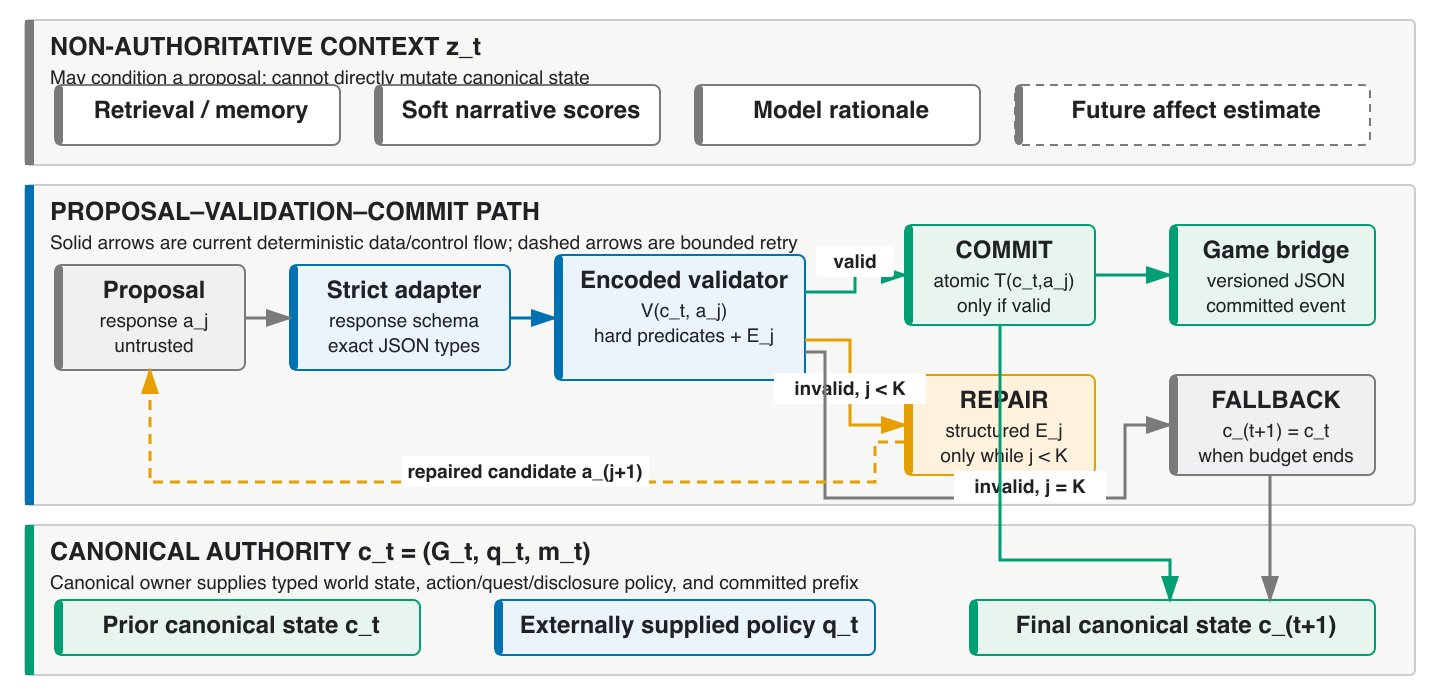
\includegraphics[width=\columnwidth]{../figures/fig_architecture.png}%
  }{\fbox{\parbox{0.9\columnwidth}{\centering Pending vector artifact: architecture and trust boundary.}}}
  \caption{Trust boundary. Retrieved context and generated candidates remain non-authoritative until known-field type checks and state-relative validation complete.}
  \label{fig:architecture}
\end{figure}

\begin{table}[t]
\caption{Encoded Validator Boundary}
\label{tab:validators}
\centering
\footnotesize
\begin{tabular}{@{}lll@{}}
\toprule
Predicate & Rejects & On failure \\
\midrule
Action policy & unknown action/type & unchanged \\
Precondition & absent/false requirement & unchanged \\
Reachability & inaccessible object & unchanged \\
NPC knowledge & undeclared known fact & unchanged \\
Disclosure & forbidden fact & unchanged \\
Quest & ineligible/regressive stage & unchanged \\
\bottomrule
\end{tabular}
\end{table}

\subsection{Validate--Repair--Commit}
The controller executes the following dependency-free pseudocode. ``Record'' denotes an append to the in-memory trace representation; persistent writing occurs only after terminal consistency checks.

\begin{figure}[t]
\footnotesize
\begin{tabular}{@{}rl@{}}
1: & $a\leftarrow\textsc{Propose}(c)$; $j\leftarrow0$ \\
2: & \textbf{repeat} \\
3: & \quad $(ok,E)\leftarrow V(c,a)$; \textsc{Record}$(a,E)$ \\
4: & \quad \textbf{if} $ok$ \textbf{then} \\
5: & \qquad \textbf{assert} $V(c,a).ok$; \textbf{return} \textsc{Commit}$(c,a)$ \\
6: & \quad \textbf{if} $j=K$ \textbf{then return} \textsc{Fallback}$(c)$ \\
7: & \quad $a\leftarrow\textsc{Repair}(c,a,E)$; $j\leftarrow j+1$ \\
8: & \textbf{until terminal}
\end{tabular}
\caption{Validate--repair--commit procedure. At most $K+1$ candidate attempts are recorded; the successful path performs a defensive validation before mutation.}
\label{alg:commit}
\end{figure}

Structured counterexamples expose error codes to a repair callback. Repair never directly mutates state, and exhaustion returns an unchanged deterministic fallback. Fig.~\ref{fig:repair} shows terminal paths.

\begin{figure}[t]
  \centering
  \IfFileExists{../figures/fig_repair_state_machine.png}{%
    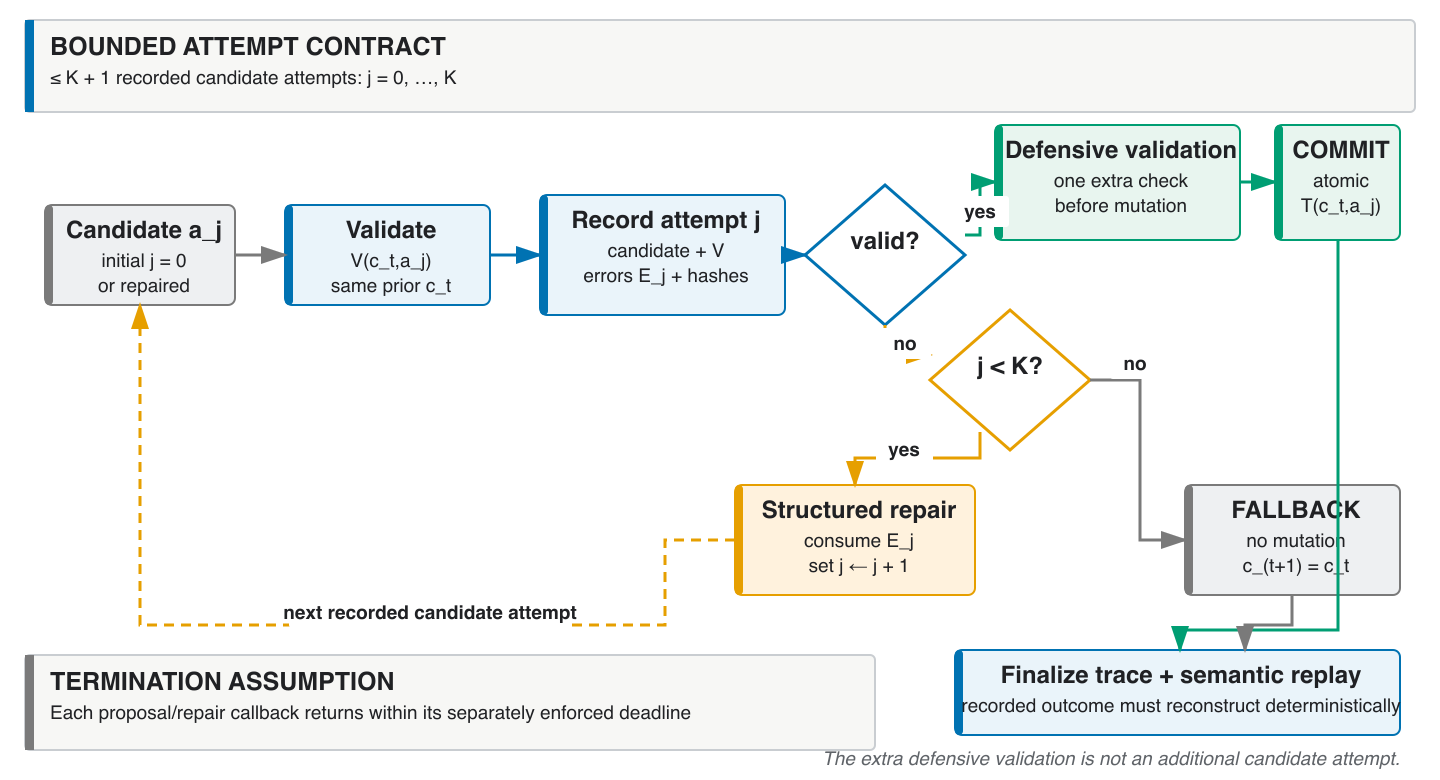
\includegraphics[width=\columnwidth]{../figures/fig_repair_state_machine.png}%
  }{\fbox{\parbox{0.9\columnwidth}{\centering Pending vector artifact: repair state machine.}}}
  \caption{Proposal, validation, bounded repair, fallback, commit, and replay states. Controller failure is terminal and may have no completed proposal trace.}
  \label{fig:repair}
\end{figure}

\subsection{Integrity, Semantic Replay, and Accounting}
Each result row carries an unkeyed SHA-256 \emph{integrity checksum}; proposal outcomes additionally link to a trace checksum. These hashes detect accidental or tested content changes but are not signatures, message-authentication codes, writer identity, or protection against an actor able to rewrite content and checksums. Semantic replay goes beyond byte integrity by strictly parsing the prior state and every recorded candidate/validation pair, requiring every nonfinal attempt to be invalid, recomputing the terminal transition, and comparing the stated final state. Episode replay also requires state continuity between adjacent JSONL records. Replay does not authenticate or re-execute the repair-generation step that produced candidate $j+1$.

The terminal record classes are commit, symbolic fallback, adapter failure, and controller failure. A controller-failure row remains in the frozen assignment denominator and leaves state unchanged, but it may legitimately lack a completed proposal trace because no candidate outcome was produced. Accordingly, result completeness does not imply trace existence for every terminal row. The pre-execution assignment key contains run, arm, scenario, seed, model, revision, controller-configuration hash, assignment-input hash, and prior-state hash. Aggregation rejects duplicate, missing, or unexpected keys and separately reports symbolic, adapter, and controller failures.

\section{Deterministic Offline Pilot Method}
\subsection{Questions and Designed Fixtures}
The pilot asks whether: (PQ1) valid candidates commit while named invalid-policy cases remain unchanged; (PQ2) rejection-only, unchanged retry, and structured repair produce the expected outcomes on authored repairable and irreparable cases; (PQ3) frozen checksum, state-semantic, linkage, and continuity mutations are rejected by their designated check operations, while an injected second-file append failure triggers the expected pair-write rollback check; and (PQ4) strict adapters and assignment manifests retain exactly one classified terminal row per assigned case or fail closed.

Cases are purposively designed conformance fixtures, not samples from a model or game population. The four domains are validator/state isolation, repair control flow, record/trace fault injection, and adapter/accounting contracts. Unique cases, rather than repeated deterministic seeds, form descriptive denominators. All expectations are specified before execution.

\subsection{Measures and Reproducibility}
Measures are exact counts: expected/observed validator-class agreement; rejected or controller-failure cases with state mutation; commit and attempt outcomes by repair arm and repairability; rejected/prespecified detectable faults by designated operation; replayed/committed traces; and rejected/injected manifest violations. Exception class alone does not identify a stable detector layer, so no detector-attribution result is reported. No $p$-values or population confidence intervals are attached to these designed fixtures. Provider-response latency in a recorded response is historical fixture metadata and is conditional on receiving a response; local adapter timing is not end-to-end game latency.

The release packet freezes fixture and assignment manifests, schemas, a result JSON artifact with embedded outcome and trace records, environment and code revision, generated tables, and checksums. Reporting follows reproducibility and measurement-boundary guidance \cite{S33_pineau2021reproducibility,S34_henderson2020energy}.

\section{Pilot Results}
\IfFileExists{../generated/pilot_results_en.tex}{%
  \subsection{Declared-Field Gate Conformance}
The pilot loader admits a fixture set only when it isolates every implemented validator code exactly once alongside one valid control, so the 13/13 agreement and the observation of all 12 implemented error codes are \emph{construction invariants of the harness}, not measured success rates. What the run adds is the part the loader does not enforce: each of the 12 isolated negative fixtures showed observed agreement with its authored expected code rather than reaching a different one, and every noncommit path preserved the complete canonical state. This is implementation conformance to an authored structured-field oracle over a single world state, not accuracy against independent semantic labels.

\subsection{Repair Mechanism}
Across two initially invalid cases, rejection-only and unchanged-candidate retry each committed 0/2. The reference repair callback committed the repairable precondition case after one repair and left the deliberately nonrepairable reachability case at fallback, for 1/2 commits. That callback is not counterexample-guided: it discards the error set and copies the policy-required preconditions and effects from the authoritative state, so it is an oracle upper bound whose outcome is determined by which candidate fields it assigns. The three arms are therefore a control-flow trace, not a comparison of repair strategies.

\subsection{Integrity, Boundaries, and Assignment Accounting}
All 10 faults prespecified as detectable were rejected by their designated check operations (10/10). Because this pilot does not compare stable typed detector codes, it does not establish detector-layer attribution. Separately, the known provenance-boundary fixture substituted a different invalid precursor before the same recorded valid repair, recomputed the checksum, and passed replay as expected (1/1 undetected). Thus, the mechanism does not protect against a writer who can recompute unkeyed checksums, and replay does not authenticate the repair-generation operation. Two open boundary sentinels---unextracted narrative disclosure and simultaneous omission of a required object from candidate and policy---were intentionally accepted at the encoded layer (2/2), with 0 labelled as safety passes. The former unknown-top-level-field acceptance boundary was reclassified after Stage 8 as a closed negative regression: both proposal and replay parsers specifically rejected a complete 12-field candidate carrying one unknown key (1/1). This establishes parser rejection parity, not semantic safety. Among seven adapter/accounting assignments, outcomes were 1 commit, 1 symbolic fallback, and 5 adapter failures. Synthetic telemetry fields were populated and propagated for 2/7 assignments; these are schema-pinned constants verifying accounting-field propagation, not measurements. All 3/3 injected duplicate or missing-assignment guards failed closed. These are raw counts from synthetic offline fixtures.
%
}{%
  \pendingartifact{\texttt{../generated/pilot\_results\_en.tex} has not yet been generated. No pilot number or empirical conclusion is inserted manually.}%
}

\IfFileExists{../generated/pilot_tables_en.tex}{%
  \begin{table}[t]
\caption{Deterministic Repair-Arm Outcomes}
\label{tab:pilot-repair}
\centering\footnotesize
\begin{tabular}{@{}lccc@{}}
\toprule
Arm & Cases & Commits & Repair calls \\
\midrule
Rejection only & 2 & 0 & 0 \\
Unchanged retry & 2 & 0 & 2 \\
Structured repair & 2 & 1 & 2 \\
\bottomrule
\end{tabular}
\end{table}

\begin{table}[t]
\caption{Frozen-Pilot Raw Accounting}
\label{tab:pilot-accounting}
\centering\footnotesize
\begin{tabularx}{\columnwidth}{@{}Xrr@{}}
\toprule
Check & Numerator & Denominator \\
\midrule
Gate fixture agreement & 13 & 13 \\
Known-boundary acceptances$^{a}$ & 3 & 3 \\
Detectable integrity faults rejected & 10 & 10 \\
Known integrity boundary replay-accepted$^{b}$ & 1 & 1 \\
Adapter commits & 1 & 7 \\
Symbolic fallbacks & 1 & 7 \\
Adapter failures & 5 & 7 \\
Manifest guards rejected & 3 & 3 \\
\bottomrule
\end{tabularx}
\vspace{1pt}\parbox{0.96\columnwidth}{\scriptsize $^{a}$Boundary acceptances document semantic-extraction, policy-completeness, and unknown-field handling limits; they are not safety passes. $^{b}$Replay does not authenticate or re-execute repair generation.}
\end{table}
%
}{%
  \pendingartifact{\texttt{../generated/pilot\_tables\_en.tex} has not yet been generated. Result tables remain evidence-gated.}%
}

\begin{figure}[t]
  \centering
  \IfFileExists{../figures/fig_evidence_boundary.png}{%
    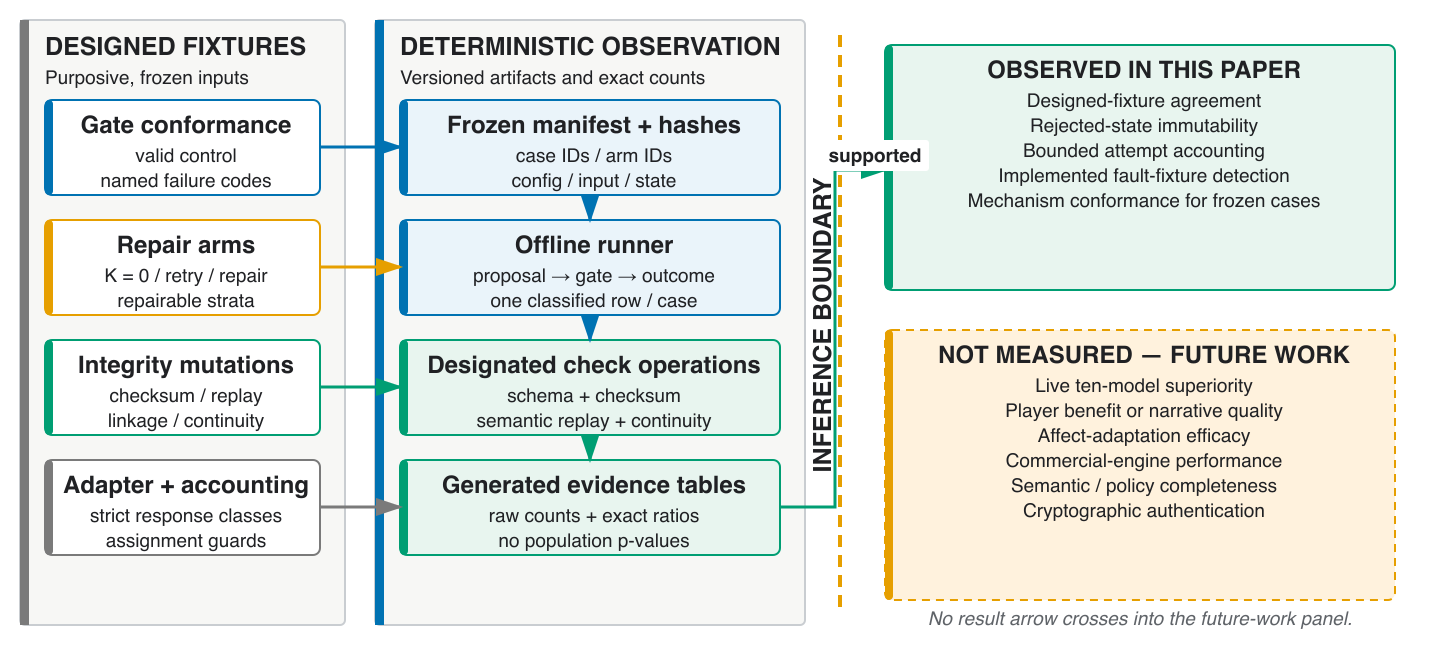
\includegraphics[width=\columnwidth]{../figures/fig_evidence_boundary.png}%
  }{\fbox{\parbox{0.9\columnwidth}{\centering Pending vector artifact: evidence boundary and fault-injection flow.}}}
  \caption{Evidence boundary from frozen fixture through a designated check operation and generated table. Counts are admitted only through generated artifacts.}
  \label{fig:evidence}
\end{figure}

Irrespective of generated counts, the pilot has no live model call, participant, affect prediction, retrieval or memory intervention, narrative-quality comparison, or actual game-engine loop. Its scope is conformance of the implemented structured transition and evidence paths.

\section{Discussion}
\subsection{Established Scope}
The designed pilot can establish mechanism behavior only for its frozen cases: whether encoded checks isolate state, whether bounded repair and fallback follow their declared paths, whether named corruptions are rejected by their designated operations, and whether assigned rows remain classified for aggregation. It does not attribute a rejection to a stable typed detector code. This is useful for authoring-time validation, continuous-integration regression, recorded-adapter tests, and pre-engine replay inspection.

The mechanism does not establish that the policy is correctly authored, that natural-language facts have been completely extracted, or that every semantically unsafe event is represented by a declared field. Nor do unkeyed hashes authenticate the writer. The writer assumes single-process ownership; concurrent-writer safety is not demonstrated. A versioned bridge is interface decoupling, not evidence of engine portability or real-time performance.

\subsection{Relationship to Prior Work}
\system{} complements constrained decoders by applying state-relative authorization after parsing \cite{S09_geng2023grammar,S10_beurerkellner2023prompting,S36_scholak2021picard}. It differs from retrieval and memory components by withholding commit authority \cite{S04_he2024gretriever,S05_gutierrez2024hipporag,S06_chhikara2025mem0}. It complements executable environments and benchmarks rather than replacing them \cite{S11_cote2019textworld,S12_wang2022scienceworld,S15_liu2024agentbench,S18_paglieri2025balrog}. Process-linked traces instantiate a measurement concern emphasized by AgentBoard \cite{S16_ma2024agentboard}; they are not evidence that \system{} outperforms that or any other system.

\section{Confirmatory Extensions}
A future registered study will screen ten frozen model instances and promote a small panel for controller comparisons. It must use an independently labelled semantic oracle, implement a genuine blind-retry comparator, record per-attempt tokens and latency, and retain timeouts and parse failures in the treatment-policy estimand. With one promoted instance per hardware/access profile, findings will remain instance-level rather than identify scale or access effects \cite{S14_perezliebana2019gvgai,S15_liu2024agentbench,S18_paglieri2025balrog,S31_agarwal2021precipice}.

Retrieval and memory ablations will compare graph and conversational-memory contexts at matched encoded validity \cite{S04_he2024gretriever,S05_gutierrez2024hipporag,S06_chhikara2025mem0}. A separate matched-validity human study will require ethics review, player-qualified raters, blinding, randomized order, attention checks, reliability, prospective power, and justified mixed-effects analysis \cite{S21_akoury2023player,S27_vanderlee2019best,S28_karpinska2021perils,S35_barr2013random}. Affect estimates will remain optional and non-authoritative; any validity non-inferiority margin requires an independent rationale \cite{S24_yannakakis2011experiencedriven,S25_melhart2020engagement,S26_wang2026engagement,S32_lakens2018equivalence}.

\section{Threats, Ethics, and Artifact Scope}
Construct validity is bounded by declared fields; an encoded check cannot discover omitted semantics. Internal validity depends on independently authored policy expectations and absence of fixture leakage. External validity is limited by offline text/mock cases. Conclusion validity is protected by reporting raw designed-case counts without population inference. Reproducibility depends on fixed software and artifact versions. Security validity is restricted to unkeyed content-integrity checks and deterministic semantic replay, not adversarial authentication.

The pilot processes no participants or personal telemetry. Future human and affect work requires applicable review, informed consent, compensation disclosure, minimization, retention/deletion rules, and opt-out. LLM judges, if used, remain auxiliary because both automated and crowd judgements require calibration and bias controls \cite{S27_vanderlee2019best,S28_karpinska2021perils,S29_zheng2023judging,S30_chen2024judgement}.

\section{Conclusion}
\system{} isolates authored candidate-event payloads from canonical mutation through an encoded neuro-symbolic commit gate and makes terminal outcomes auditable through linked records and state-semantic replay. The deterministic offline pilot is evidence about the implemented mechanism in frozen fixture domains, not cross-model superiority, player-experience benefit, retrieval or memory effectiveness, affect efficacy, or commercial-engine performance. These remain explicit confirmatory extensions.

\bibliographystyle{IEEEtran}
\bibliography{../references}

\end{document}
